
\chapter{今後の課題:提案手法の遅延}
\label{sec:appendix3}
本研究における未解決の課題である,提案手法におけるウェイクアップ時の遅延に関して説明する.

提案手法にはウェイクアップ論理の遅延が増加するという問題がある.これは,ウェイクアップ論理のクリティカル・パスに SVSD での SVS の生成と,タグの高位ビットと SVS との論理積が加わるためである.一般に,ウェイクアップ論理はプロセッサ全体のクリティカル・パスであるため,ウェイクアップ論理の遅延増加は,クロック・サイクル時間の増加につながり,結果として性能が低下する.したがって,提案手法によるウェイクアップ論理の遅延の増加は許容できる範囲に抑える必要がある.

SVSD での遅延の影響を評価するために,HSPICE による回路シミュレーションにより測定を行った.16nm LSI プロセスを仮定し,トランジスタ・モデルとして,アリゾナ州立大学のPredictiveTechnology Model(PTM)~\cite{model2012}を使用した.International Technology Roadmap for Semi-conductors(ITRS)~\cite{itrs2012}により公開されているデータより,単位長さあたりの配線抵抗は 46.96MΩ/m,配線容量は 0.165nF/m とした.なお,この HSPICE による回路シミュレーションは,松田~\cite{matsuda-thesis}の作成したネットリスト生成プログラム及び遅延測定用スクリプトを修正して使用することにより行った. 

測定を行った SVSD 回路の回路図を\fig{SVSD_nand_nor}に示す.同図は,セグメント数が 8 で,タグのビット数が 8 ビットの場合を示している.基本的な回路構成は\refsec{segment_IQ}で説明したものと同様であるが,CMOS トランジスタで構成するため,NAND 及び NOR を使用する回路構成に変更している.本回路に関して詳しく説明する.

\ctext{1}SVSD は,デスティネーション・タグの下位 3 ビットの正転及び反転信号を用いて,セグメント数分の SVS の反転信号($\lnot SVS\;0$ 〜 $\lnot SVS\;7$)を生成する.\ctext{2} SVS の反転信号は,デスティネーション・タグ(dtag3 〜 dtag7)の反転(正転)信号と NOR をとり,SVS によって有効化されたデスティネーション・タグ(V-dtag:Validated dtag)の正転(反転)信号を生成する.これは,以下の論理式に基づいている.
\[
  V\mathchar`-dtag = \lnot (\lnot dtag \lor \lnot SVS) \; (= dtag \land SVS) 
\]
\[
  \lnot V\mathchar`-dtag = \lnot (dtag \lor \lnot SVS) \; (= \lnot dtag \land SVS) 
\]
生成された V-dtag は各セグメントに送られ,セグメント内の 全エントリの CAM に入力される.

松田のネットリスト生成プログラムを修正して,SVS を含む提案手法のウェイクアップ回路の遅延測定を行った.測定結果を\tab{delay}に示す.表の各項目は次の意味を持つ.
  \begin{itemize}
    \item from tagRAM:タグRAM から SVS  の入力までの遅延.
    \item SVS:SVS 信号を生成するまでの遅延(\fig{SVSD_nand_nor}における赤い矢印).
    \item broadcast:SVS により有効化したタグが CAM に到達するまでの遅延(\fig{SVSD_nand_nor}における青い矢印) .
  \end{itemize}
 
  \begin{table}[htb]
    \caption{タグ RAM 出力からタグ放送までの遅延時間(ps)}
    \footnotesize
    \center
      \begin{tabular}{l|l} \hline \hline
       from tagRAM & 22 \\
       SVS & 36 \\
       broadcast & 106 \\ \hline
      合計 & 164 \\ \hline
    \end{tabular}
    \label{tab:delay}
  \end{table}

 同表において,合計値は,提案手法を用いない通常の IQ における,タグ RAM 出力からタグ放送までの遅延時間の遅延時間に該当する.通常の IQ におけるタグ RAM 出力からタグ放送までの遅延時間を測定したところ,105ps 程度であった.したがって,提案手法によってブロードキャストの遅延時間が 60ps 程度増加していることが分かる.これは,無視できないほど大きな遅延の増加である.
  
  この主な要因は,SVS による遅延時間の増加であると考える.SVSD は 3 入力の NAND ゲート 1 つ分の遅延であるため,その遅延時間はそこまで大きくないはずである.しかし,測定結果は 36ps と遅延時間が大きい.この原因は特定できていないが,おそらく SVSD の NAND ゲートへの入力信号の立ち上がりが遅いためではないかと予測している.

  この問題に対しては,以下の対処方法が有効である可能性がある.
  \begin{itemize}
  \item タグ RAM に SVSD を配置し, SVS に変換してからブロードキャストする
  \item ディスパッチ時にあらかじめ SVS にデコードしてタグ RAM に記録しておき,ウェイクアップ時にタグとともにブロードキャストする
  \end{itemize}
  これらの方法について検討し,ウェイクアップ論理の遅延増加を許容できる範囲に抑えることが今後の課題である.
  
\begin{figure}[htb]
  \centering
  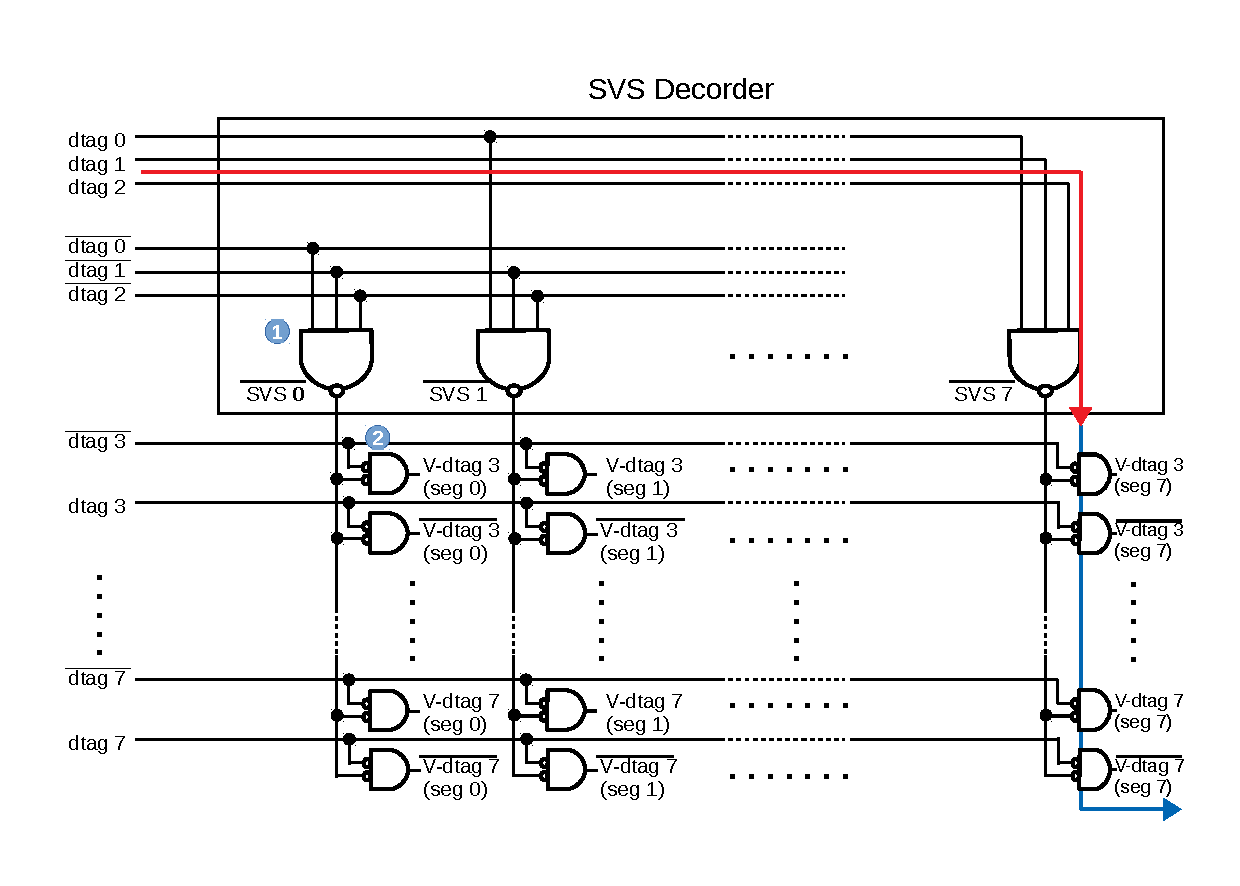
\includegraphics[keepaspectratio, scale=.8]{SVSD_nand_nor}
  \caption{SVSD(遅延評価用)}
  \label{fig:SVSD_nand_nor}
\end{figure}
